\documentclass[12pt]{article}
\usepackage[spanish]{babel}
\usepackage{graphicx}
\usepackage{mathtools}

\begin{document}

\section{Primer sección}
Esto es un texto de relleno sin sentido. La figura \ref{fig:leon}, el cuadro \ref{tab:datos} y la ecuación \eqref{eq:ecuacion}.

\begin{figure}[h]
	\centering
	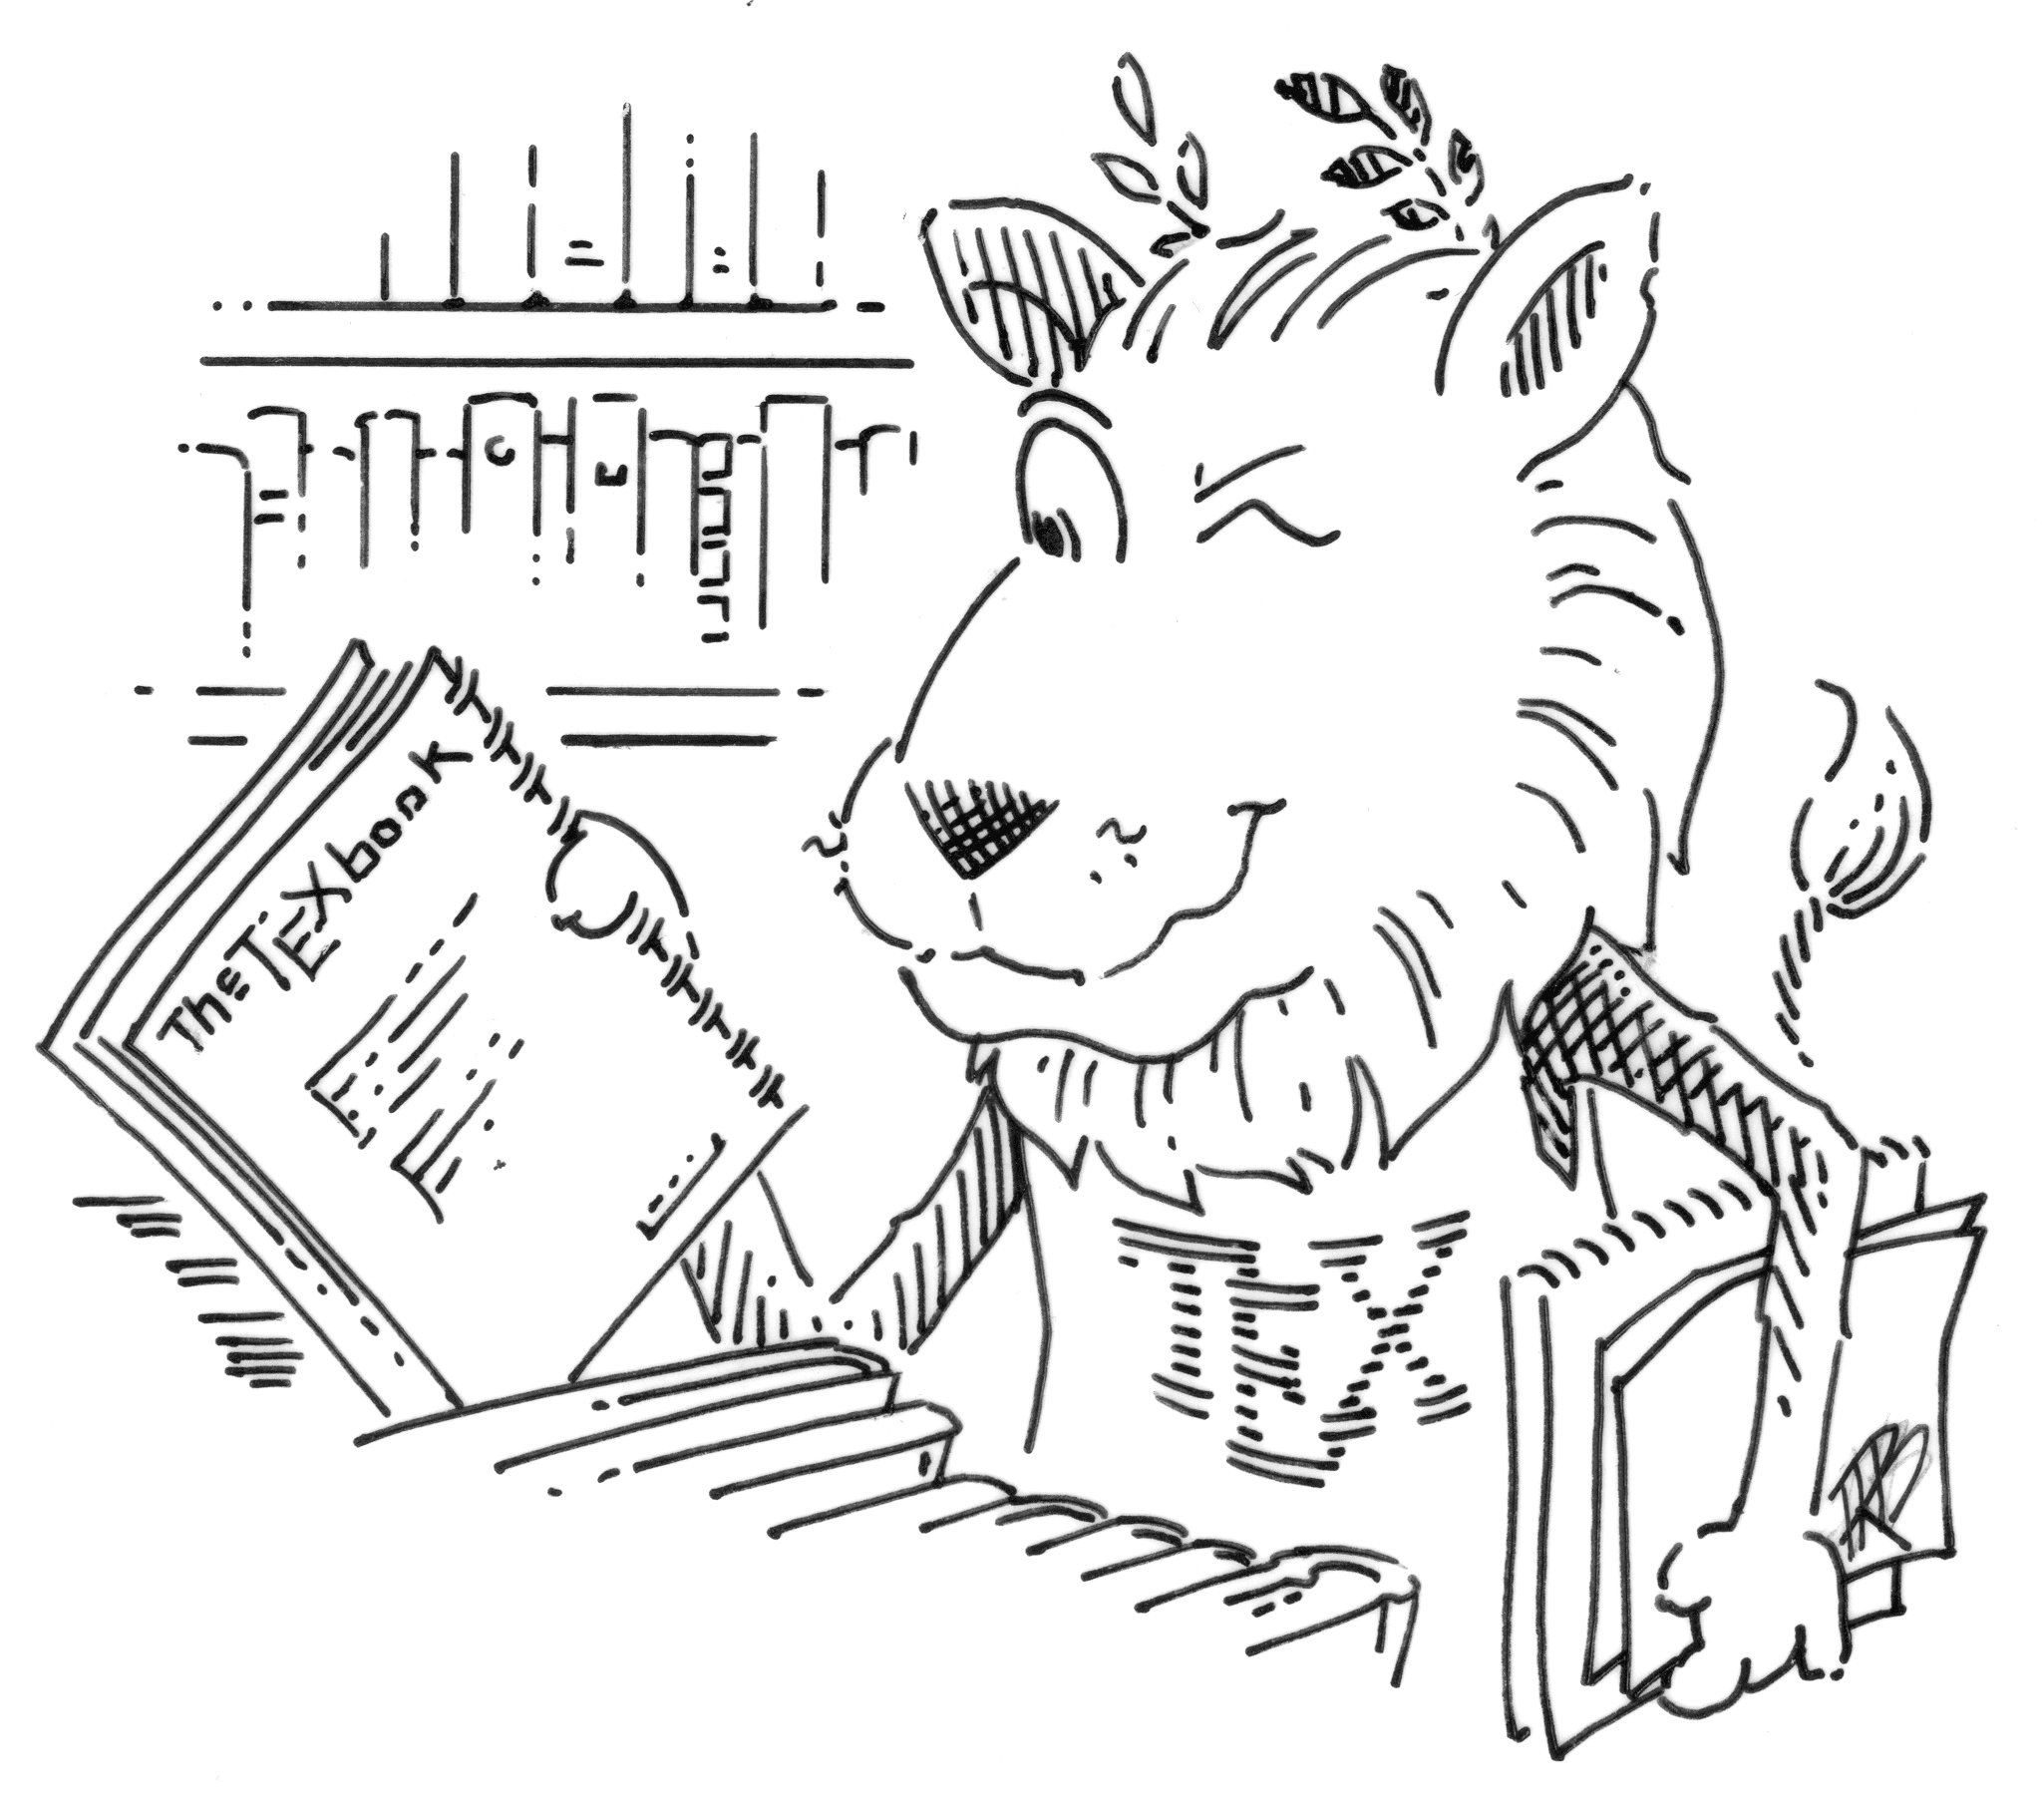
\includegraphics[width=0.4\linewidth]{figuras/leon}
	\caption{Esto es una leyenda.}
	\label{fig:leon}
\end{figure}

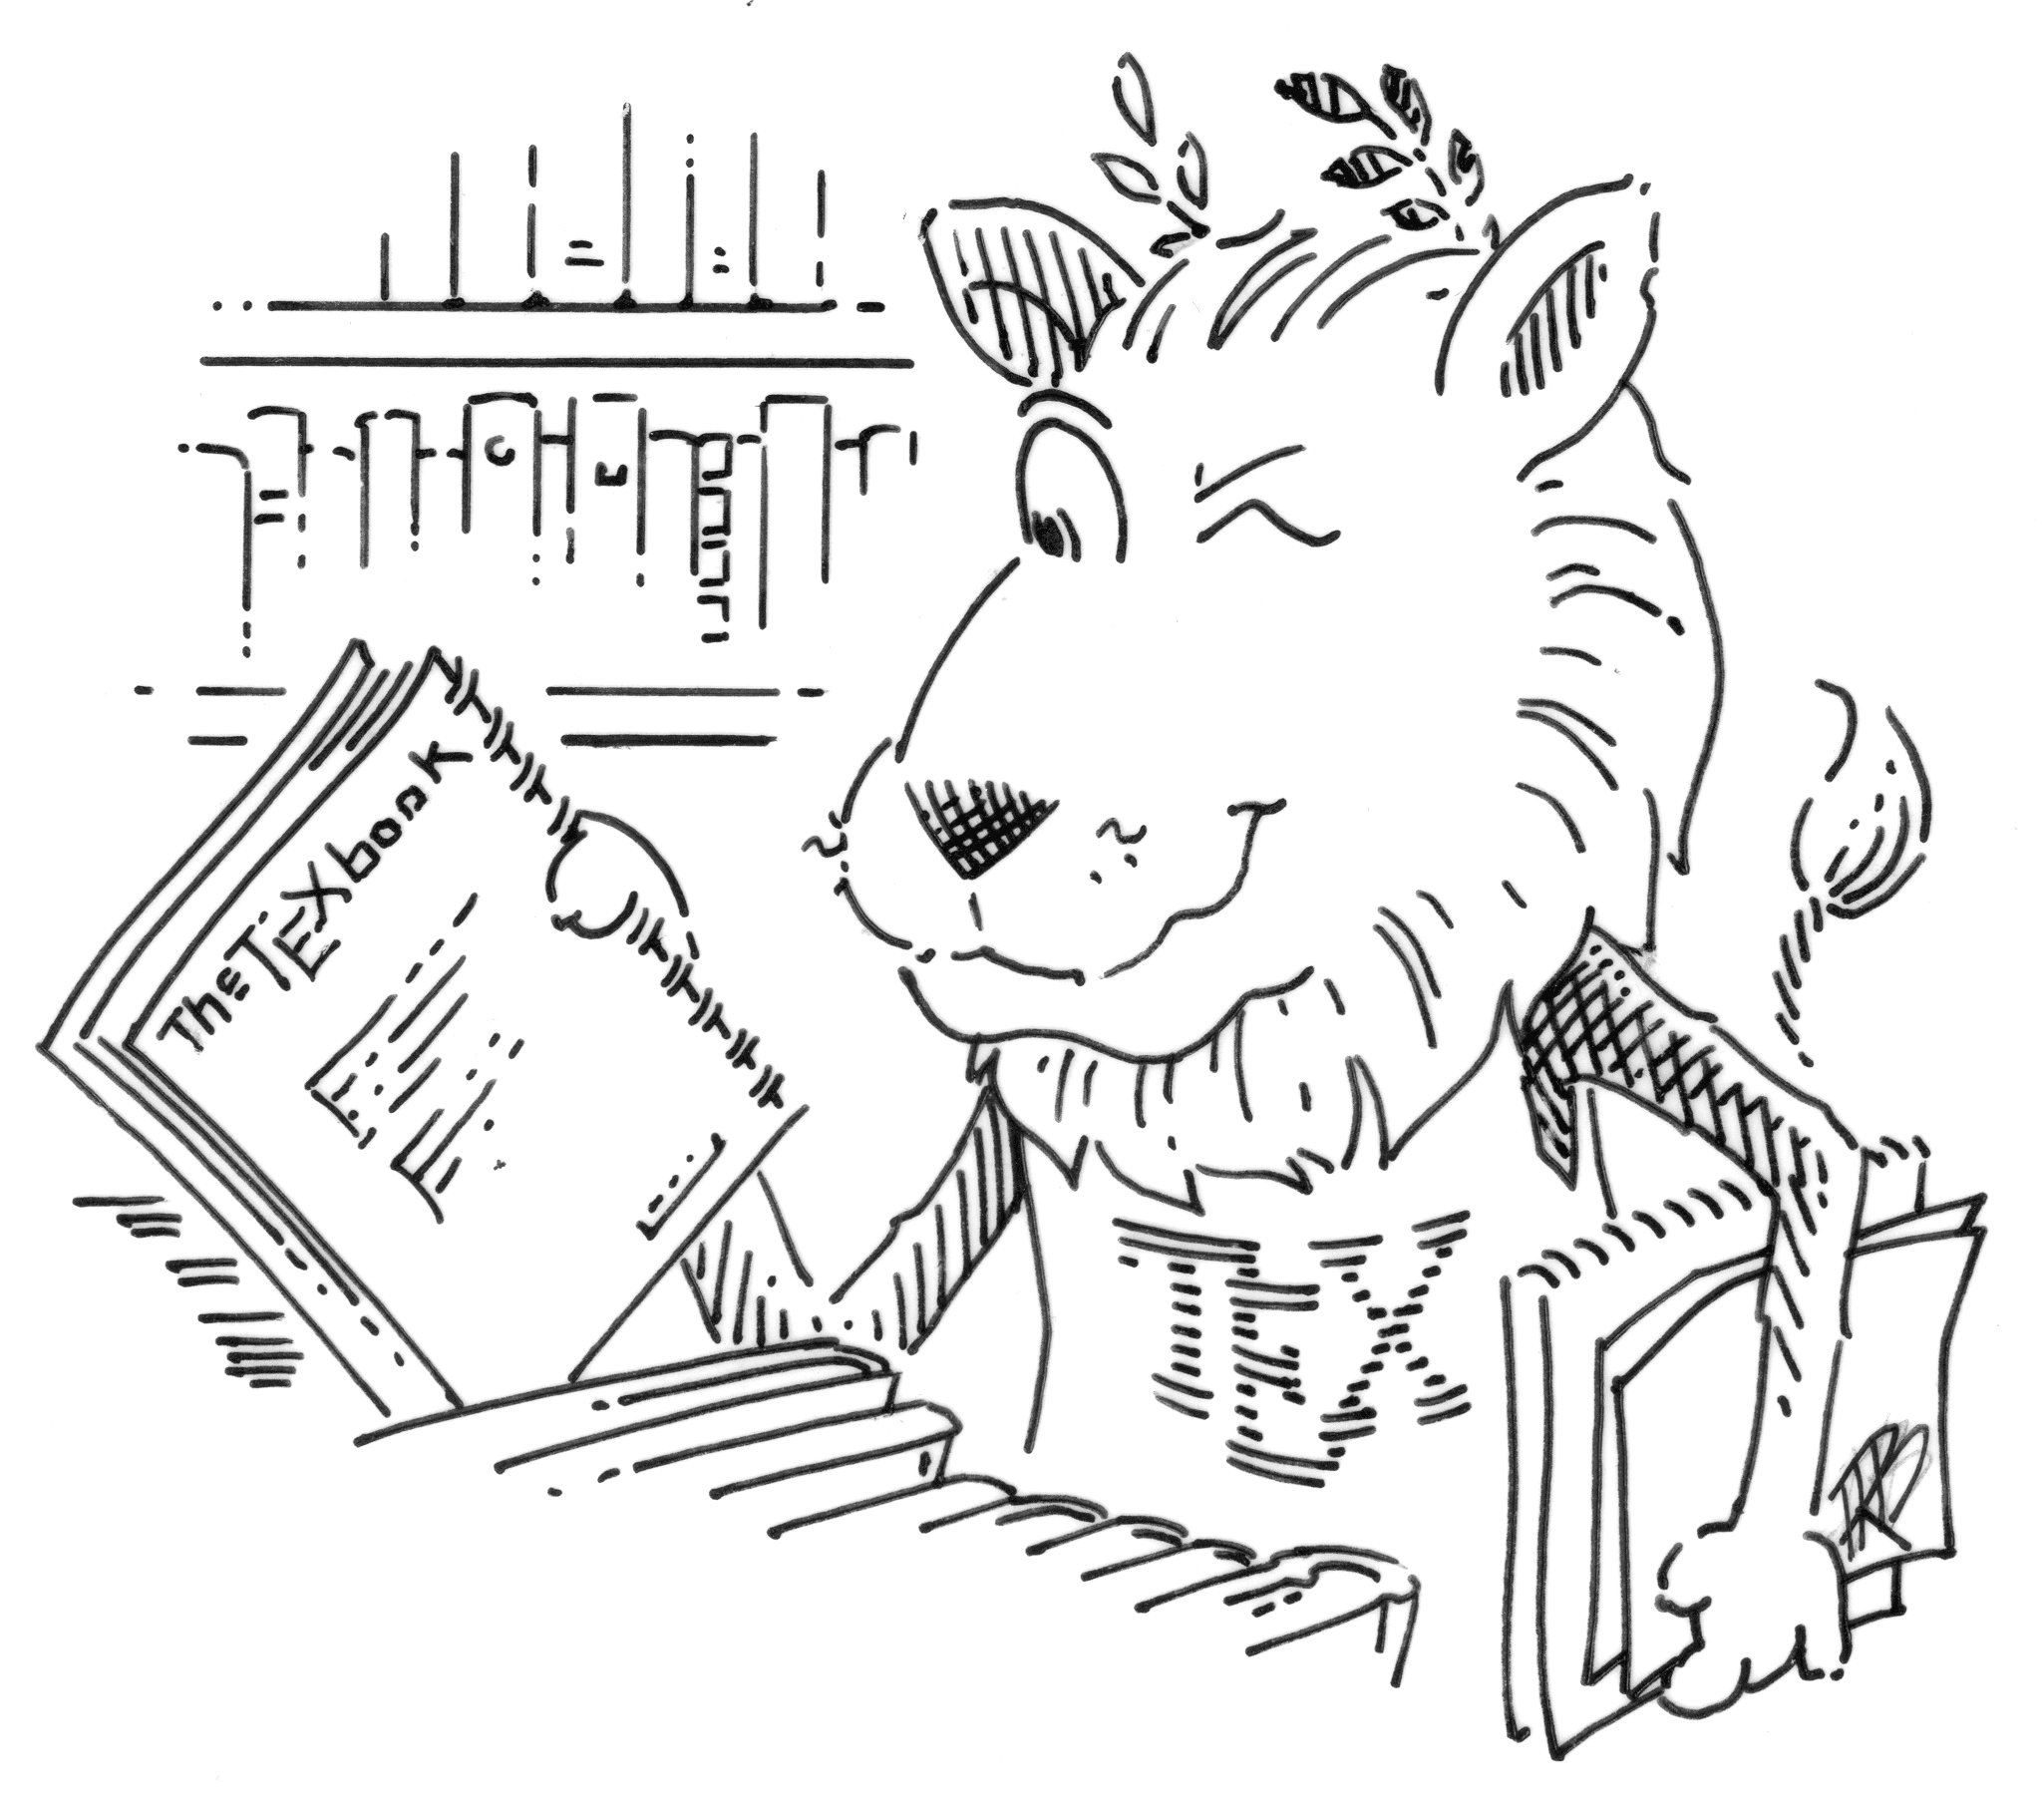
\includegraphics[width=0.4\linewidth]{figuras/leon}

	\begin{tabular}{|l|c|r|}
	\hline
	hola & 23 & 2 \\
	\hline
	1 & hola & 3 \\
	\hline
	2 & 5 & hola \\
	\hline
\end{tabular}

\begin{table}[h]
	\centering
	\caption{Esto es una leyenda.}
	\begin{tabular}{|l|c|r|}
		\hline
		hola & 23 & 2 \\
		\hline
		1 & hola & 3 \\
		\hline
		2 & 5 & hola \\
		\hline
	\end{tabular}
	\label{tab:datos}
\end{table}

Esta es una ecuación $x^2 \Rightarrow y$. $\sum _{i=0}^{n}f{\left(x\right)}^{2}=0$. $E = m\cdot c^2$

\begin{equation} \label{eq:ecuacion}
	E = m\cdot c^2
\end{equation}


\end{document}
